% Created 2019-09-05 jeu. 17:57
% Intended LaTeX compiler: pdflatex
\documentclass[presentation]{beamer}
\usepackage[utf8]{inputenc}
\usepackage[T1]{fontenc}
\usepackage{graphicx}
\usepackage{grffile}
\usepackage{longtable}
\usepackage{wrapfig}
\usepackage{rotating}
\usepackage[normalem]{ulem}
\usepackage{amsmath}
\usepackage{textcomp}
\usepackage{amssymb}
\usepackage{capt-of}
\usepackage{hyperref}
\RequirePackage{fancyvrb}
\DefineVerbatimEnvironment{verbatim}{Verbatim}{fontsize=\scriptsize}
\usetheme{default}
\author{Laurent Garnier}
\date{\today}
\title{Feuille de route pour créer un smart contract}
\hypersetup{
 pdfauthor={Laurent Garnier},
 pdftitle={Feuille de route pour créer un smart contract},
 pdfkeywords={},
 pdfsubject={},
 pdfcreator={Emacs 26.2 (Org mode 9.1.9)}, 
 pdflang={English}}
\begin{document}

\maketitle
\begin{frame}{Outline}
\tableofcontents
\end{frame}


\begin{frame}[fragile,label={sec:orgf034b04}]{Structure générale du dossier}
 Dans tout dossier chaincode il doit y avoir :
\begin{itemize}
\item un fichier nommé \texttt{chaincode.yaml}
\item un dossier \texttt{src}
\item dans le dossier \texttt{src} il doit y avoir :
\begin{enumerate}
\item Le code source \texttt{nom\_du\_fichier.go}
\item L'API de description \texttt{openapi.yaml}
\end{enumerate}
\end{itemize}

Voir la figure ci-dessous :

\begin{center}
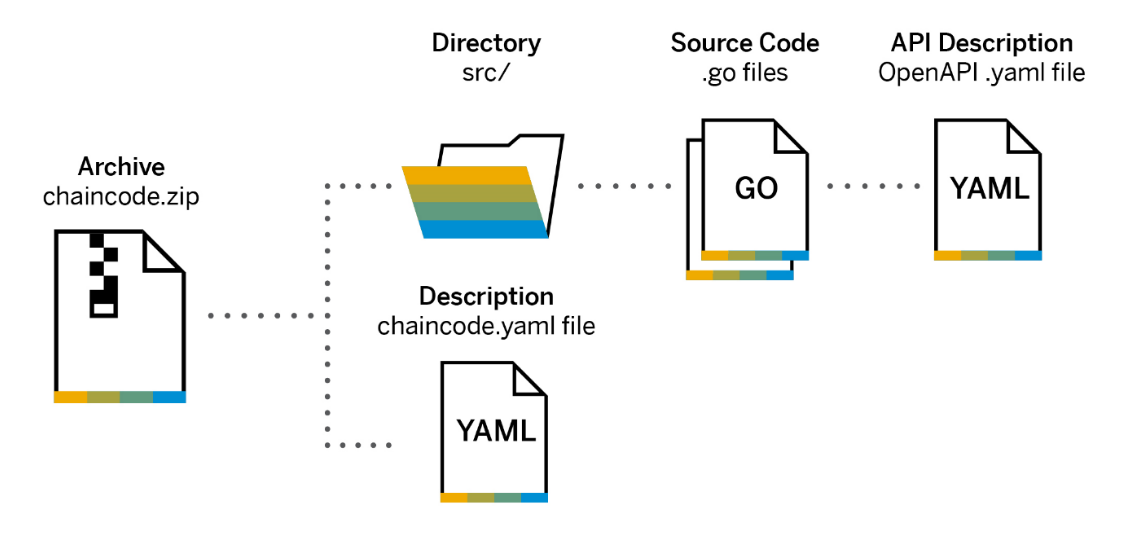
\includegraphics[width=.9\linewidth]{./chaincode_dir_struct.png}
\end{center}
\end{frame}

\begin{frame}[fragile,label={sec:org86f5e09}]{Le fichier \texttt{chaincode.yaml}}
 Dans ce fichier nous fournirons les méta-données de notre chaincode.

Les balises Id et Version sont importantes ici. 

Chaque fois qu'un chaincode est appelé, soit depuis une API REST soit depuis un autre chaincode, l'identifiant (ID) 
du chaincode doit être connu. 

Cet ID doit aussi être fourni lorsque le chaincode est déployé.

Nous recommandons de spécifier tous les IDs de chaincode dans le format DNS inverse, comme pour les classes Java.

Par exemple, l'Id de notre chaincode est \texttt{blockchain-example-chaincode\_test}.

Cette syntaxe pour les IDs de chaincode : caractères alphanumérique et les tirets - et \_.

De la même manière, chaque chaincode se voit attribué un numéro de version.

Puisqu'un chaincode est déployé "pour toujours" sur la blockchain et ne peut être effacé, pour remplacer 
un chaincode on ré-utilise sont numéro de version.

Durant le déploiement, le numéro de version doit être disponible. 
\end{frame}

\begin{frame}[fragile,label={sec:orge515de1}]{Code du fichier \texttt{chaincode.yaml}}
 \begin{verbatim}
# THIS SAMPLE CODE MAY BE USED SOLELY AS PART OF A TEST 
# BLOCKCHAIN SERVICE (THE "SERVICE") AND IN ACCORDANCE 
# WITH THE TERMS OF THE AGREEMENT FOR THE SERVICE.
# THIS SAMPLE CODE PROVIDED "AS IS", WITHOUT ANY WARRANTY, 
# ESCROW, TRAINING, MAINTENANCE, OR SERVICE OBLIGATIONS 
# WHATSOEVER ON THE PART OF ALMERYS/BE|YS.

Id:       blockchain-example-chaincode_test
Version:  1
\end{verbatim}
\end{frame}

\begin{frame}[fragile,label={sec:orgedf4284}]{Création du fichier de description API}
 ALMERYS/BE|YS fournit une porte d'entrée qui expose toutes les fonctions chaincode comme des APIs REST normales.

Vous pouvez accomplir cela en fournissant une description OpenAPI de l'API REST qui est liée aux fonctions du chaincode.

Vous faites cela avec le document YAML qui est écrit avec le chaincode en golang.

Le document YAML décrit exactement comment chaque fonction peut accédée via un appel REST, quels paramètres sont disponibles
et comment les paramètres doivent être transmis au chaincode.

Dans le dossier \texttt{src} créer un fichier \texttt{hello\_world.yaml} :
\end{frame}

\begin{frame}[fragile,label={sec:org8dbcb06}]{Code du fichier \texttt{hello\_world.yaml}}
 \begin{verbatim}
swagger: "2.0"
info:
  description: |
    The Hello World! chain code shows the first steps 
    in developing a chaincode that can read/write 
    strings onto the blockchain and can expose these 
    functions as REST API. 
    THIS SAMPLE CODE MAY BE USED SOLELY AS PART OF 
    THE TEST AND EVALUATION OF THE ALMERYS/BE|YS 
    BLOCKCHAIN SERVICE (THE "SERVICE") AND IN 
    ACCORDANCE WITH THE AGREEMENT FOR THE SERVICE. 
    THIS SAMPLE CODE PROVIDED "AS IS", WITHOUT ANY 
    WARRANTY, ESCROW, TRAINING, MAINTENANCE, OR 
    SERVICE OBLIGATIONS WHATSOEVER ON THE PART OF 
    ALMERYS/BE|YS.
  version: "1.0"
  title: "Hello World!"
\end{verbatim}
\end{frame}

\begin{frame}[label={sec:orgd92886e}]{Création du fichier du code source (en Golang)}
Lors du développement d'un chaincode, l'étape suivante est d'écrire le programme 
GO lui-même (ce qui est notre chaincode).

Dans le programme, il peut y avoir un nombre quelconque de fonctions, chaque 
fonction ayant un nombre quelconque de paramètres "non nommés".

L'appelant de toute fonction doit connaître le nom de la fonction et de la séquence 
exacte de paramètres. 

Dans les configurations Hyperledger Fabric standards, l'accès au chaincode se fait 
uniquement via un SDK ce qui requiert un accès du chaincode au HTTPS/gRPC.
\end{frame}

\begin{frame}[fragile,label={sec:org50984d2}]{Code du fichier \texttt{hello\_world.go} :}
 \begin{verbatim}
// DISCLAIMER:
// THIS SAMPLE CODE MAY BE USED SOLELY AS PART OF THE TEST 
// AND EVALUATION OF THE ALMERYS/BE|YS BLOCKCHAIN SERVICE 
// (THE "SERVICE") AND IN ACCORDANCE WITH THE TERMS OF THE 
// AGREEMENT FOR THE SERVICE. THIS SAMPLE CODE PROVIDED 
// "AS IS", WITHOUT ANY WARRANTY, ESCROW, TRAINING, 
// MAINTENANCE, OR SERVICE OBLIGATIONS WHATSOEVER ON THE 
// PART OF ALMERYS/BE|YS.
\end{verbatim}
\end{frame}

\begin{frame}[fragile,label={sec:org2076334}]{Comprendre le fichier de description API}
 Le fichier de description API \texttt{hello\_world.yaml} est utilisé pour décrire l'interface
HTTP exacte pour le chaincode.

C'est important de comprendre que le fichier \texttt{.yaml} est ensuite utilisé dans deux 
contextes différents : 
\begin{itemize}
\item Pour générer la page de test API depuis laquelle les APIs de chaincode peuvent 
être testées directement
\item La passerelle d'API utilise des aspects spécifiques du fichier YAML pour décider 
de la méthode d'extraction des paramètres de la requête HTTP entrante. Ensuite, 
ils associent ces éléments à une fonction du chaincode à appeler.
\end{itemize}
\end{frame}
\begin{frame}[fragile,label={sec:orgc096e6e}]{Comprendre la correspondance verbes HTTP et appels de chaincode}
 Un ensemble riche de verbes HTTP est utilisé de manière spécifique pour que 
les appels REST imitent les opérations CRUD (Create Read Update Delete) typiques
des bases de données.

Du côté Hyperledger Fabric, les fonctions chaincode peuvent être appelées comme suit : 

\begin{itemize}
\item Par un appel \texttt{Invoke} qui écrit une transaction avec des ensembles lecture/écriture 
dans la blockchain
\item Par un appel \texttt{Query} pour un type de fonction en lecture seule
\end{itemize}


Pour toutes les demandes HTTP entrantes, chaque verbe HTTP spécifique correspond à un 
appel Invoque ou Query de Hyperledger Fabric.

Dans cet exemple de chaincode, nous utiliserons des appels POST et GET.
\end{frame}

\begin{frame}[label={sec:org62533f6}]{Tableau des correspondances HTTP/Chaincode}
\begin{center}
\begin{tabular}{llll}
Verbe HTTP & Action type & Correspond à & Effet sur la Blockchain\\
\hline
POST & Créer & Invoke & Ecrit une transaction\\
\hline
GET & Lire & Query & Aucun\\
\end{tabular}
\end{center}
\end{frame}




\begin{frame}[fragile,label={sec:orgc8928b7}]{Comprendre les chemins de chaincode}
 La section des chemins de chaincode est utilisée pour définir une définition 
enrichie de l'API basée sur REST et toutes les fonctionnalités de Swagger 
peuvent être utilisées pour décrire l'API. Deux cas spéciaux s'appliquent : 

\begin{itemize}
\item Pour chaque chemin, vous devez préciser l'\texttt{operationId}. C'est le nom de direct de la 
fonction chaincode qui doit être appelée pour ce chemin.
\item Pour les paramètres, les cinq emplacements de paramètres sont pris en charge. Les paramètres
peuvent être \texttt{path}, \texttt{query}, \texttt{header}, \texttt{form}, ou \texttt{body}. Pour les types de paramètres, 
vous pouvez utiliser uniquement des paramètres simples qui peuvent être mis en correspondance
avec des type de chaîne de caractères en entrée de chaincode. Les types acceptés sont : 
\texttt{string}, \texttt{number}, \texttt{integer}, \texttt{boolean}, et \texttt{file}.
\end{itemize}
\end{frame}

\begin{frame}[fragile,label={sec:org3cd54aa}]{Définir le chemin du chaincode de \texttt{POST}}
 Pour définir le chemin d'accès au chaincode (utilisé pour appeler le chaincode), 
ouvrir le fichier \texttt{hello\_world.yaml} avec un éditeur de texte et copiez-collez les lignes suivantes :
\end{frame}

\begin{frame}[fragile,label={sec:org1fda918}]{Code du fichier \texttt{hello\_world.yaml}}
 \begin{verbatim}
consumes:
  - application/x-www-form-urlencoded

paths:

  /{id}:

    post:
      operationId: write
      summary: Write a text (once) by ID
      parameters:
      - name: id
	in: path
	required: true
	type: string
      - name: text
	in: formData
	required: true
	type: string
      responses:
	200:
	  description: Text Written
	500:
	  description: Failed
\end{verbatim}
\end{frame}

\begin{frame}[fragile,label={sec:org197fcd7}]{Explications}
 Ce chemin de publication (\texttt{POST}) inclut la fonction write (\texttt{operationID: write}), deux paramètres pouvant être écrits 
(\texttt{id} et \texttt{text}) et deux codes de réponse (200 pour la réussite de la publication et 500 pour l'échec).

Notez que cet exemple inclut également la section \texttt{consumes}. 

Ceci définit les types de contenu par défaut qui seront acceptés pour tous les appels d'API, s'ils ne sont pas définis 
spécifiquement. Par défaut, il doit être défini sur \texttt{application/x-www-form-urlencoded} pour signaler que les demandes 
HTTP entrantes auront des paramètres au format nom / valeur.
\end{frame}
\begin{frame}[fragile,label={sec:org69a2f90}]{Définir le chemin \texttt{GET}}
 Pour définir le chemin de chaincode \texttt{GET} (utilisé pour interroger le chaincode), 
copiez et collez les lignes suivantes sous le code précédent :
\end{frame}





\begin{frame}[fragile,label={sec:org8f6c452}]{Code du fichier \texttt{hello\_world.yaml}}
 \begin{verbatim}
get:
     operationId: read
     summary: Read text by ID
     parameters:
     - name: id
       in: path
       required: true
       type: string
       produces:
     - text/plain
     responses:
       200:
	 description: OK
       500:
	 description: Failed
\end{verbatim}
\end{frame}
\begin{frame}[fragile,label={sec:orge9b4988}]{Explications}
 Ce chemin pour \texttt{GET} comprend les fonctions de lecture (\texttt{operationID: read}), 
un paramètre à lire (\texttt{id}) et deux codes de réponse (200 pour une lecture 
réussie et 500 pour un échec de lecture).
\end{frame}
\begin{frame}[fragile,label={sec:org91c28db}]{Valider le \texttt{hello\_world.yaml} avec Swagger.io}
 Ouvrir un navigateur web et naviguer jusqu'à l'éditeur \href{https://editor.swagger.io/}{Swagger.io}

Cliquer sur File > Clear Editor

\begin{center}
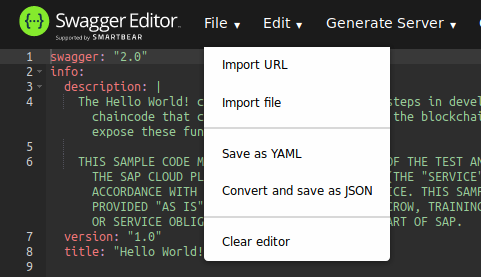
\includegraphics[width=.9\linewidth]{./swagger_file_clear.png}
\end{center}

Puis copier le code du fichier \texttt{hello\_world.yaml} à l'intérieur
\end{frame}

\begin{frame}[label={sec:orgcbbe311}]{Swagger complet}
\begin{center}
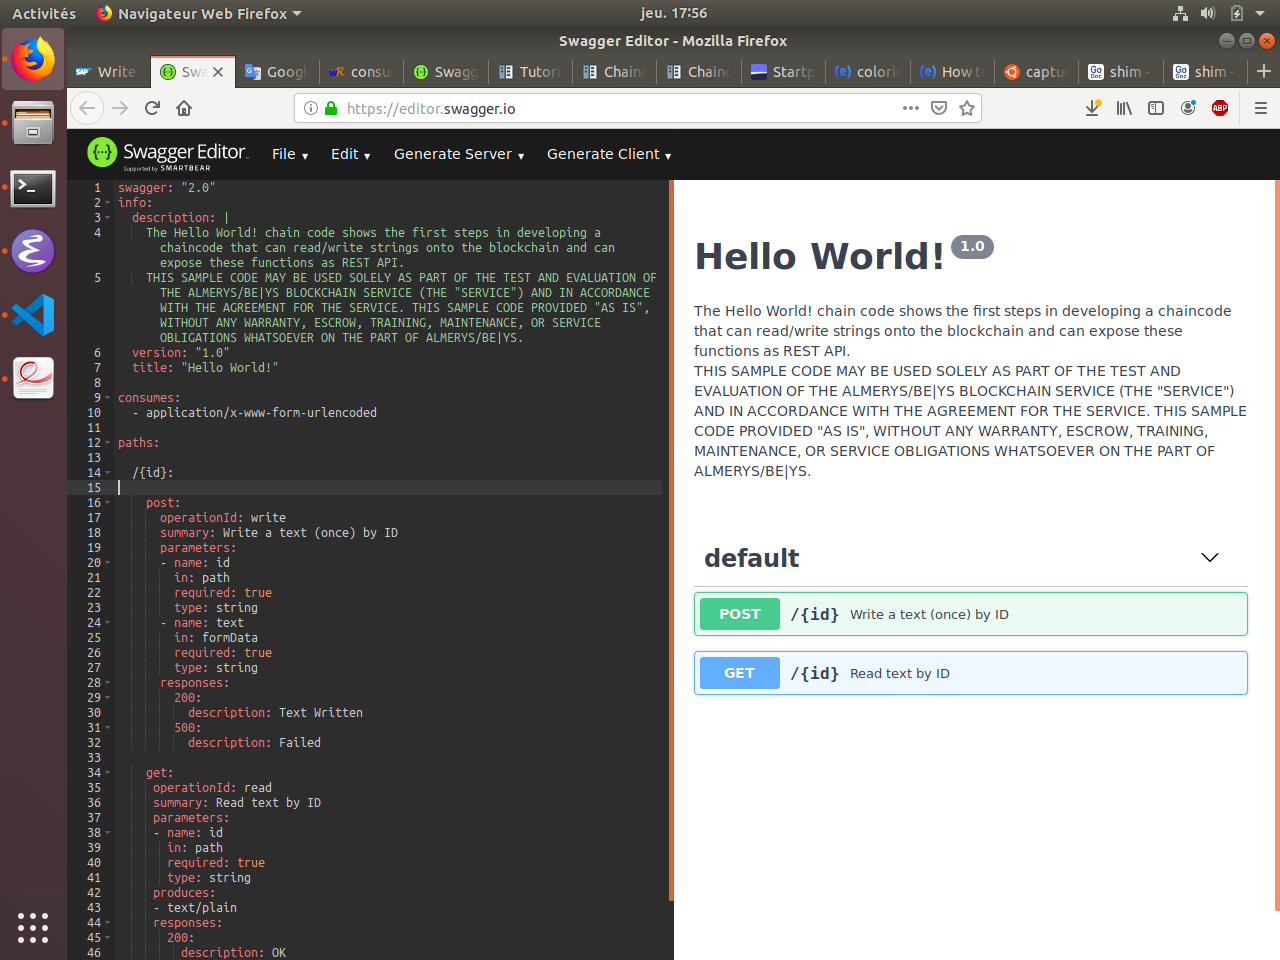
\includegraphics[width=.9\linewidth]{./swagger_complete.png}
\end{center}
\end{frame}
\end{document}
